\section{Introduction}\label{sec:Introduction}

\subsection{Purpose and Structure of this Document}

This document presents the System Specification for an Information and
Monitoring Services middleware component (R-GMA), in sufficient detail to
support the following activities:

\begin{itemize}
  \item Design verification: This document sets out precisely \textit{what
  R-GMA will do}, so that it can be verified that it will provide the required
  services to other middleware components and Grid users.
  
  \item System design: Detailed designs will show exactly
  \textit{how} the system specified here will be implemented.
  
  \item System test: This document is the primary input to test
  specification activities.
\end{itemize}

This chapter is followed by one describing message formats then
a separate chapter for each of the R-GMA services, with a standard set of
headings in each chapter. Chapters on security, SQL language support, service data types and service parameters
complete the document.

\subsection{Concepts}
\subsubsection{Virtual Database}
R-GMA enables Grid users to share information in a \textit{virtual
database\index{virtual database}\index{database!virtual|see{virtual database}}
(VDB)\index{VDB|see{virtual database}}}. To the ordinary user a
virtual database looks much like a real one. It organises its data
into tables, and data can be inserted and queried using standard SQL
constructs. It even supports indexes and views. However there is no
central repository holding the data for each table. A virtual database
just consists of a list of table definitions (called a
\textit{schema}\index{schema}), a list of data providers (called a
\textit{registry}\index{registry}) and a set of rules for deciding
which data providers to contact for any given query. These rules are
fixed by R-GMA, and are encoded into a hidden component called the
\textit{mediator} and described in section \ref{sec:Consumer}.

\begin{center}
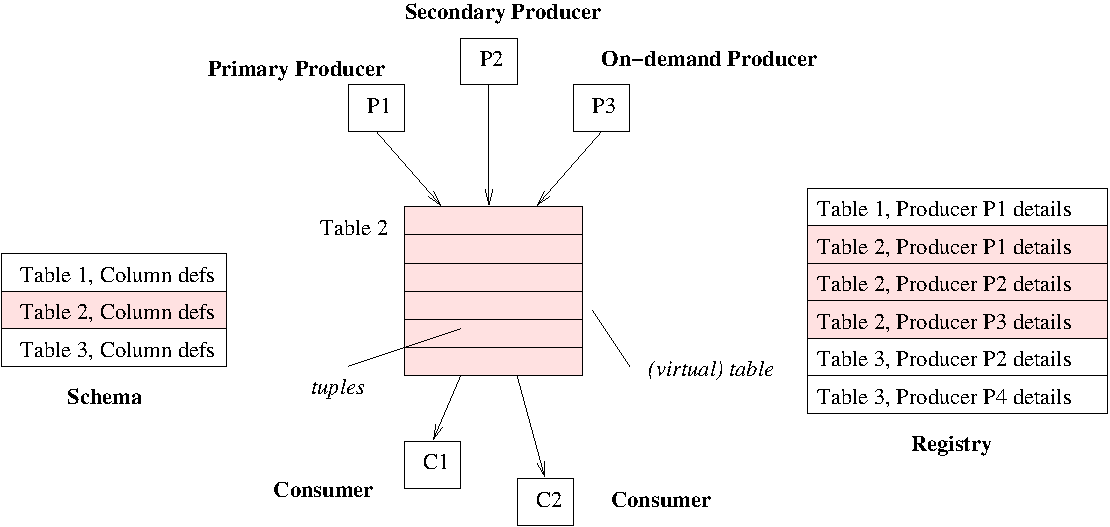
\includegraphics[width=155mm]{virtual_db}
\end{center}

The picture above shows the principal components of R-GMA. Data is written into 
the virtual database by \textit{producers} and read from it by 
\textit{consumers}. The model used by R-GMA, where consumers contact the 
registry to obtain a list of producers for their query then contact the 
producers directly to get the data, is known as the Grid Monitoring 
Architecture (GMA) and was first described by the Open Grid Forum (or Global
Grid Forum as it as at that time).

A single Grid can support any number of virtual databases. Each
virtual database has a Grid-wide unique name. Typically, a virtual
database will be owned and managed by a \textit{virtual
organization}\index{virtual organisation} (VO)\index{VO|see{virtual
organisation}}, but R-GMA doesn't require this to be the case.

R-GMA is not a distributed database management system. Instead, it
provides a useful and predictable information system built on a much
looser coupling of data providers across a Grid. This document
provides a precise description of that information system.

\subsubsection{Producers}

Producers\index{producer} are the data providers for the virtual
database. Writing data into the virtual database is known as
\textit{publishing}, and data is always published in complete rows,
known as \textit{tuples}\index{tuple}.  There are three classes of
producer: \textit{Primary}\index{primary
producer}\index{producer!primary|see{primary producer}},
\textit{Secondary}\index{secondary
producer}\index{producer!secondary|see{secondary producer}} and
\textit{On-demand}\index{on demand producer}\index{producer!on
demand|see{on demand producer}}. Each is created by a user application
and returns tuples in response to queries from consumers. As the
picture below shows, the main difference is in where the tuples come
from.

\begin{center}
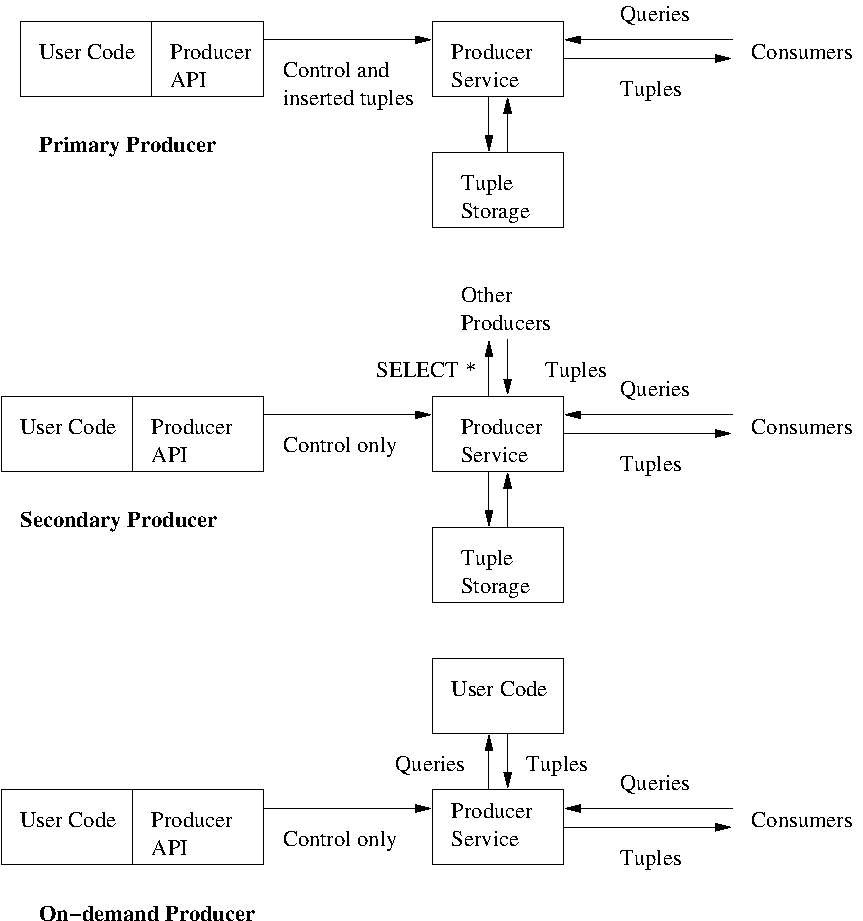
\includegraphics[width=115mm]{producers_overview}
\end{center}

The \textit{producer service} in these pictures is a process running
on a server, acting on behalf of the user code (this is explained in
the Services Architecture in section~\ref{sec:wsa}). In a Primary
Producer, the user code periodically inserts tuples into storage
maintained internally by the producer service. The producer service
autonomously answers consumer queries from this storage. The Secondary
Producer service also answers queries from its internal storage, but
it populates this storage itself by running its own query against the
virtual database: the user code sets the process running and the
tuples come from other producers. In the On-demand Producer, there is
no internal storage; data is provided by the user code in direct
response to a query forwarded to it by the producer service.

The tuple storage maintained by Primary and Secondary producers can
either be in memory or in a real database. Producers that use
memory storage are optimized to answer simple queries quickly,
but they must still be able to answer the same queries as producers using
database storage, even if that means creating an in-memory database on the fly.
In an On-demand producer, tuple storage, if any, is outside of R-GMA and is
the responsibility of the user code.

\subsubsection{Consumers}

In R-GMA, each consumer\index{consumer} represents a single SQL SELECT
query on the virtual database. The request is initiated by user code,
but the \textit{consumer service} carries out all of the work on its
behalf. The query is first matched against the list of available
producers in the Registry and a set of producers capable of answering
the query is selected, in a process called \textit{mediation}. The
consumer service then sends the query directly to each selected
producer to obtain the answer tuples.

\begin{center}
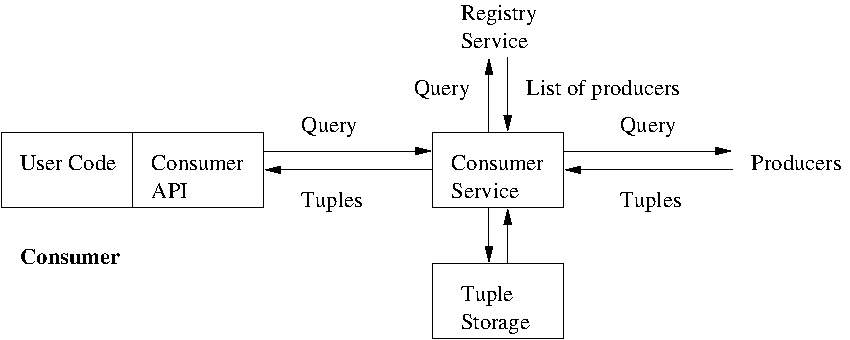
\includegraphics[width=115mm]{consumer_overview}
\end{center}

\subsubsection{Query types}\label{sec:BackgroundQueryTypes}

There are four types of query: \textit{continuous}\index{continuous
query}\index{query!continuous|see{continuous query}},
\textit{latest}\index{latest query}\index{query!latest|see{latest
query}}, \textit{history}\index{history
query}\index{query!history|see{history query}} and
\textit{static}\index{static query}\index{query!static|see{static
query}}. The set of queries that a particular producer supports is
recorded in the registry. All query types except static can take an
optional time interval parameter.

All four types of query cause tuples to be streamed
from producer services to the consumer service that is running the
query on the consumer application's behalf. The consumer application
can then pull the tuples from the consumer service in its own time.

Continuous queries are subscriptions\index{subscription} with
producers to receive all \textit{new} tuples that match the query;
tuples are streamed to the consumer service automatically as they are
inserted into the virtual database by the Primary producers.
Streaming continues until the consumer requests it to stop.
Continuous consumers are also registered in the Registry so they can
be notified if the list of relevant producers changes during the
lifetime of the query. If a time interval is specified, the producers
selected for streaming will additionally send any tuples they already
have, that are not older than the time interval.
There is no guarantee that tuples are time-ordered.
All Primary and Secondary producers support continuous queries.
On-demand producers do not.

Latest and history queries are \textit{one-time}
queries\index{one-time query}\index{query!one-time|see{one-time
query}}: they are evaluated against the current contents of the
virtual database, the results are streamed back to the consumer
service, and then they terminate. In a history-query, all versions of
any matching tuples are returned; in a latest-query, only those
representing the ``current state'' (see below) are returned. In both
cases, a time interval may be specified with the query, to limit the
age of the tuples returned, as in a continuous query. Primary and
Secondary Producers may optionally support one-time queries. On-demand
producers do not.

Static queries are one-off database queries and are only supported by
On-demand producers. The purpose of On-demand producers is to make
external data stores accessible through the R-GMA infrastructure so it's
unlikely that an On-demand producer will publish to the same table as Primary
and Secondary producers.

\subsubsection{Tuple Management}\label{sec:BackgroundTupleManagement}

All tables in an R-GMA schema have several metadata columns added to the
table definition by R-GMA when the table is created in the schema (see
\ref{sec:PrimaryProducerInserting} for the column definitions). These columns
are filled in when tuples are inserted into a Primary producer and include a
time-stamp added by R-GMA if the user has not already done so.
Secondary producers do not modify tuple metadata in the tuples they republish.
On-demand producers put null values into the metadata columns of all tuples
they publish.

Primary and Secondary producers have one or two tuple stores, 
a \textit{history tuple store} against which history queries are evaluated (and 
from which tuples are retrieved for continuous queries), and an optional 
\textit{latest tuple store} against which latest queries are evaluated. 
On-demand producers do not store tuples.

Each tuple inserted into a primary or secondary producer added to the 
producer's history tuple store, regardless of what is already there: no attempt 
is made to detect duplicates. If applicable, it is also added to the producer's 
latest tuple store, provided it is not older than any previous version already 
there, which means its time-stamp must be no earlier than any tuple with the 
same \textit{primary key} that is already in the tuple-store. If an older 
version exists, it is replaced by the new one. The primary key is a subset of 
the columns in the table, and is defined when the table is first created in the 
schema. This is the only place in R-GMA where the the primary key is used.

Primary producers declare a \textit{Latest Retention
Period}\index{Latest Retention Period}~\textit{(LRP)}\index{LRP|see
{Latest Retention Period}} on each table to which they publish
tuples.  The LRP is used by the primary producer to calculate a \textit{latest
retention time} for each tuple, by adding the LRP to the tuple's
time-stamp. This is stored in the tuple's metadata and remains unaltered
when the tuple is republished by a Secondary Producer. A latest-query is evaluated against only the most recent versions of
tuples, and only those tuples that have not exceeded their latest
retention time (this is the definition of current state).

Both primary and secondary producers declare a \textit{History Retention
Period}\index{History Retention Period}~\textit{(HRP)}\index{HRP|see
{History Retention Period}} on each table to which they publish
tuples. The HRP is considered to be relative to the time at which the tuple is
stored in the producer and is not relative to the time stamp on a tuple.
A history-query is evaluated against whatever is available, but that
is guaranteed to include at least all versions of tuples that have not
exceeded the producer's HRP for the table.

Retention periods do not affect the delivery of tuples to continuous consumers:
it is fundamental to the mediation logic of R-GMA that its producer services
ensure that all new tuples are streamed to all subscribed consumers, unless
there is an unrecoverable fault that prevents it.

Producers are obliged to periodically remove expired tuples from their tuple
stores so that they do not run out of storage space. The exact details of how
retention periods work for each producer type
are specified in the corresponding chapters in this document.

\subsection{Service Architecture}\label{sec:wsa}\index{Service Architecture}
\subsubsection{Services}

R-GMA is implemented as a set of six types of \textit{service} running on one or
more servers. They are Primary Producer, Secondary Producer, On-demand Producer,
Consumer, Registry and Schema.  The virtual database is realised by the
interaction of these services; users contact their local services to publish data
or run queries on the virtual database, and the service translates this into a
sequence of operations to be carried out locally, or by contacting other R-GMA
services as necessary, on their behalf. Each service has a well defined set of
\textit{operations} that are requested by applications through an exchange of
messages with the service. The semantics of the operations and their parameters
are defined in  subsequent chapters in this  document. The operations in each
service are grouped into \textit{user operations} and \textit{system operations}.
User operations are used by client applications and (some) by other R-GMA
services. System operations are used by other R-GMA services only.

R-GMA uses https calls in a request/response pattern, for all user-to-service 
and service-to-service communications apart from streaming.  Streaming tuples 
to continuous consumers uses a lower level communication protocol, for 
efficiency (see section~\ref{sec:PrimaryProducerQueryProcessing}).

\subsubsection{Resources}\index{resource}

Connections to R-GMA services only last for the duration of a single
operation, but in producer and consumer services, R-GMA needs to
retain private data \textit{between} operations, for each producer or
consumer instance currently being managed by the service. In a Primary
or Secondary producer, for example, this includes the tuple
stores.  R-GMA stores the private data
associated with each producer and consumer in a \textit{resource}. It
is created by the service when a user calls a ``create'' operation and
is given an identifier that is passed back to the client. The client
then includes the resource identifier with all subsequent requests
relating to this resource. Resource identifiers are positive integers
that are unique within any given service and are not re-used.  A
resource is normally closed/destroyed at the explicit request of the user,
but in order to protect itself from an accumulation of redundant
resources, an R-GMA service requires the user to periodically contact
the service to keep the resource alive. A resource has a 
\textit{termination interval};  if the service doesn't hear
from the user for any period exceeding the termination interval, the resource is
closed by the service. For most purposes the APIs hide the need to know about
termination intervals - though the server can be queried to discover what
termination intervals are being used.

The registry protects itself in a similar way, against producers and consumers that
register then disappear, so a periodic message is also
sent to the registry by the consumer and producer services, on the
user's behalf to keep the producers and consumers registered.

\subsubsection{Service APIs}\index{API}

R-GMA provides APIs for Java, C++, C and Python languages, to make it
easier for user applications to interact with the R-GMA services.  The
APIs are independent of each other and are designed to present an
apropriate interface to R-GMA for each supported language.  Each API
contains a method for each user operation of every service, and that
method simply packages up its parameters into an https request and
sends it to the service for execution. Any return values or errors are
passed back to the caller. The API transparently manages any
authentication required by the server, and looks after the resource
identifier.

All R-GMA services report errors\index{error handling} by sending 
exceptions\index{exception}, which are described fully in 
\ref{sec:BackgroundErrorReporting}. Each API presents service and API 
exceptions to the user in a manner appropriate to the language, for example as 
Java Exceptions. The absence of an exception indicates success. The results of 
SQL queries (tuples) are returned in \textit{tuple sets}.

The server may report to the API that a resource is no longer available. In this
case it is the responsibility of the API to create a new resource in the same
state as the old one. In the case of a consumer a warning is attached to the
next tuple set so that the user is made aware as some data loss may have
occured.

\subsubsection{Service Security}\index{security}

Security for R-GMA is discussed in detail, in
section~\ref{sec:Security}.  

\subsection{Fault Tolerance}\index{fault tolerance}
\subsubsection{Registry and Schema Replication}

The schema\index{schema replication}\index{replication!schema|see{scheam 
replication}} and registry\index{replication!registry|see{registry 
replication}}\index{registry replication} represent the only single point of 
failure in a virtual database, so multiple replicas are maintained in different 
Registry and Schema services in the Grid. Each service can host the registries 
and schemas of multiple virtual databases. Replicas are synchronized according 
to the rules in sections~\ref{sec:RegistryReplication} 
and~\ref{sec:SchemaReplication}. Users, producer services and consumer services 
always contact their local Registry and Schema services, and it's the 
responsibility of those services to locate working replicas and switch as 
necessary following failure.

\subsubsection{Service Failure and Recovery}\index{failure}\index{recovery}

R-GMA producer and consumer resources are always destroyed when the
service hosting them stops or restarts. All calls to services in R-GMA, either
from the user or another service, must therefore be prepared to
discover that a resource no longer exists, or is no longer registered in the
registry, and to handle the error gracefully. The use of time-outs (soft-state
registration) in the registry ensures entries
for resources that no longer exist are automatically removed within a
reasonable length of time.

Those R-GMA services that use permanent storage (registry service,
schema service and primary and secondary producers with permanent
tuple stores (see, for example,~\ref{sec:PrimaryProducerTupleStores})) do have
some degree of resilience, because new resources
can reconnect to existing storage, provided the storage itself is
recoverable.  In the case of the registry and schema, the database is
brought up to date by the replication mechanisms. In the case of a permanent
tuple-store, a producer created using the existing store will automatically
make tuples already in the tuple-store available to consumers, and they
will remain in the store until they exceed their retention period, in
the usual way. Backing up permanent storage (e.g. database backups)
is outside the scope of R-GMA's responsibility.

\subsubsection{Traffic Jams}

Processing a single operation in R-GMA can involve interactions
between several services. In addition, each service can expect to
handle a large number of simultaneous client requests. It can also be
expected that at any one time there may be a number of clients and
services that are slow to respond or even block completely. R-GMA
service implementations must ensure therefore, through the use of
queues, thread pools, connection timeouts and other devices, that all
correctly functioning clients and services get a reasonable response,
and a small number of blocked connections are not able to seriously
disrupt the overall operation of the service. Deliberate attempts to disrupt a
service (denial-of-service attacks) are discussed in the chapter on security.

\subsubsection{Clock Synchronization}\index{synchronisation of clocks}

As far as possible relative rather than absolute times are passed between
R-GMA servers however some absolute times are passed so any servers running
R-GMA services should keep their clocks synchronized using a protocol such as NTP.

\subsubsection{Error reporting}\label{sec:BackgroundErrorReporting}\index{error handling}

R-GMA services use the following exceptions for reporting all
errors.

\begin{description}


\item[RGMAPermanentException] Any kind of error when it is unlikely that
repeating the call will lead to success. This might be caused for example by bad
parameters in the call from the user or a corrupt database.
\item[RGMATemporaryException] An error where it is probable that repeating the
call may be sucessul. This might be caused by memory being low or the server
becoming too heavily loaded.
\item[UnknownResourceException] Resource identifier
is unknown. This will not be passed back to the user via the API but the API will
create a new resource.
\end{description}

RGMAPermanentException and RGMATemporaryException are implemented as subclasses of
RGMAException by those API languages that support the concept.

In the case of fatal errors, external resources (especially database
and network connections) are freed up and any threads associated with
the resource are terminated as cleanly as possible.

Warnings\index{warning} are only issued in R-GMA in response to
consumer queries, and only to indicate possible inadequacies in the
results. They are appended to the query's result set.

\subsection{Bootstrapping}\label{sec:BackgroundBootstrapping}\index{bootstrapping}

R-GMA servers run all R-GMA services. Users only have to be able to locate and 
connect to a single server, usually at their own site to avoid 
firewall\index{firewall} problems, in order to use R-GMA. All APIs locate these 
services using a file containing their URLs that is configured when the APIs 
are installed, and is unlikely to change.

Producer and Consumer services only connect to other Producer and Consumer 
services through URLs passed to them in system calls, or to the Registry and 
Schema services on their own server. The Registry and Schema services will act 
as proxies if requests need to be forwarded to other Registry and Schema 
services.

Registry and Schema services need to be able to locate other Registry and 
Schema services, firstly to be able to forward requests to virtual databases 
that they're not hosting locally, and also to be able to replicate the 
registries and schemas that they are hosting locally. They obtain this 
information from files that maps virtual database names to Registry and Schema 
service URLs for all virtual databases supported at that site.
